\chapter{Analyse mit CryptoMiniSat}
\label{chp:analyse}

Die im letzten Kapitel erstellte konjunktive Normalform wird in diesem Kapitel für eine Analyse mit CryptoMiniSat verwendet.
Analyse bedeutet in diesem Fall, Lösungsversuche mit CryptoMiniSat durchzuführen. CryptoMiniSat sammelt dabei zusätzliches Wissen
in Form von Konfliktklauseln. Außerdem können durch die Optimierung der ursprünglichen konjunktiven Normalform weitere Klauseln
generiert werden. Sowohl die Konfliktklauseln als auch die aus der Optimierung entstandenen Klauseln sollen in diesem Kapitel
analysiert werden um die Module aus dem vorhergehenden Kapitel mit weiterem Wissen anzureichern und weitere Lösungsversuche zu
beschleunigen. Das Vorgehen ist dabei iterativ. Nach einem Lösungsversuch werden mutmaßlich wertvolle Klauseln identifiziert
und in die Module aufgenommen, um mit diesem zusätzlichen Wissen einen weiteren Lösungsversuch zu starten.

Als Lösungsversuch wird die Urbildberechnung (siehe Abschnitt \ref{sec:urbildberechnung}) herangezogen. Die Initialwertberechnung
(siehe Abschnitt \ref{sec:initialwertberechnung}) eignet sich nicht, da die Eingabe bekannt ist und somit die Erweiterung der Eingabe
vollständig berechnet werden kann. Dadurch ist dieser Teil bereits gelöst und wird im Lösungsversuch nicht berücksichtigt. Das führt
dazu, dass kein Wissen über die Erweiterung der Eingabe erworben werden kann. Für die Urbildberechnung wird der Hash aus Abbildung
\ref{fig:ruby-sha256} herangezogen. Dieser wurde aus der Eingabe "`Das ist eine Eingabe aus der ein Hash erstellt wird."' mit Hilfe
der interaktiven Rubykonsole berechnet und dient unter anderem auch als Testfall für die Kompressionsfunktion. Ziel des Lösungsversuchs
ist es, eine Eingabe mit 52 Byte Länge zu finden. Dies könnte auch die Eingabe sein, die benutzt wurde um den Hash zu berechnen.
\begin{figure}[!h]
  \centering
  \begin{lstlisting}[]
  require 'digest'
  Digest::SHA256.hexdigest 'Das ist eine Eingabe aus der ein Hash erstellt wird.'
                        => "27931f0e7e53670ddbec1a1ce23e21b4663c63c0d17117ee1a934bc0c294dbe9"
  \end{lstlisting}
  \caption{Ruby - \glos{sha256}}
  \label{fig:ruby-sha256}
\end{figure}

Beachtet werden muss auch, dass der Hash nicht direkt mit in die konjunktive Normalform kodiert wird. Gleiches gilt für die Initialwerte
und das Padding, was vorgegeben wird um die Eingabelänge zu definieren. Eine direkt Kodierung würde dazu führen, dass erworbenes Wissen
sich auf diese Werte bezieht und somit nur für diesen Fall gültig ist. Um das zu vermeiden werden alle Werte als "`Annahmen"' (Assumptions)
an CryptoMiniSat übergeben. Das führt dazu, dass die Werte zwar für diesen Lösungsversuch gelten, jedoch nicht als allgemeingültig betrachtet
werden. Klauseln die auf diesem Wissen basieren, werden separat behandelt und nach dem Lösungsversuch verworfen.

Ebenfalls berücksichtigt werden muss die Extraktion der gelernten Klauseln aus CryptoMiniSat. Die internen Datenstrukturen sind nicht dafür
geeignet, die Klauseln während eines laufenden Lösungsversuchs zu extrahieren. Eine Extraktion kann nur erfolgen, wenn CryptoMiniSat eine
Lösung gefunden hat wobei die Lösung auch sein kann, dass es keine Lösung gibt. Wie zu erwarten ist, kommt CryptoMiniSat aber bei vollständiger
Vorgabe des Hash zeitnah zu keiner Lösung. Deshalb wird ein iterativer Ansatz verfolgt. Die Initialwerte und das Padding werden immer vollständig vorgeben,
während die Vorgabe des Hash bitweise erweitert wird. Nach jeder Lösung werden dabei die Klauseln extrahiert. Es werden so lange Bits des Hash
ergänzt, bis keine Lösung mehr gefunden wird. Im Allgemeinen zeigt sich dies dadurch, dass CryptoMiniSat aufgrund eines vollen Hauptspeichers
abstürzt oder das Programm selbst die Menge der Klauseln nicht mehr handhaben kann.

Extrahiert werden in jedem Lösungsversuch die irredundanten und die redundanten Klauseln. Die irredundanten Klauseln enthalten zunächst die
eingegebene konjunktive Normalform, die jedoch während der Lösungsversuche optimiert wird. Die redundanten Klauseln enthalten das gelernte
Wissen, das zusätzlich genutzt wird und wegfallen könnte, ohne die Lösungsmenge zu beeinflussen.

In den folgenden Abschnitten wird die Analyse der extrahierten Klauseln im Detail beschrieben. Zunächst werden in Abschnitt \ref{sec:ana:rem_double}
alle Klauseln gesammelt und schon bekannte Klauseln aussortiert. In Abschnitt \ref{sec:ana:module} wird versucht, die Klauseln einzelnen Modulen
zuzuordnen und diese zu normalisieren. Gelingt die Zuordnung zu einem Modul nicht, wird in Abschnitt \ref{sec:ana:distance} eine Distanzmetrik
genutzt, um die Klauseln zu bewerten und mutmaßlich wertvolle Klauseln zu identifizieren und zu verallgemeinern. Durch die Iterationen, die jeweils
gelerntes Wissen mit einbeziehen, kann es dazu kommen, dass Dont-Care Literale identifiziert werden und zur Verkürzung von Klauseln führen.
Diese Entwicklung wird in Abschnitt \ref{sec:ana:generalize} betrachtet. Abschließend wird das gelernte Wissen in Abschnitt \ref{sec:ana:acquired}
zusammengefasst. \TODO{Diesen Absatz an tatsächliche Struktur anpassen}

\section{Aussortieren bekannter und doppelter Klauseln}

\TODO{erledigen}

ganz einfach. kein wissensgewinn\\
c++ set\\
bekanntes aussortieren um ermitteltes wissen zu gewinnen\\
bekannt ist die kombination aus mit und ohne xor
\section{Erkennen und normalisieren modulspezifischer Klauseln}
\label{sec:ana:module}

Nach dem Aussortieren der schon bekannten Klauseln werden die neuen Klauseln den einzelnen Modulen zugeordnet. Durch die hierarchische Anordnung
muss beachtet werden, dass eine Klausel mehreren Modulen zugeordnet werden kann. Sinnvoll ist es jedoch, die Klausel nur dem Modul zuzuordnen
das in der Hierarchie möglichst weit unten steht. Wird eine Klausel für einen Addierer gefunden, kann diese Klausel so zukünftig für alle Addierer
genutzt werden, während sie im Modul für die vollständige Kompressionsfunktion nur für den einen speziellen Addierer gelten würde. Um diese
Zuordnung zu realisieren erhält jedes Modul ein Level. Im hierarchischen Aufbau muss das Level eines Moduls dabei höher sein, als das höchste Level
der verwendeten Module. Die vergebenen Level sind in Abbildung \ref{fig:sha256_module_level} dargestellt.
\begin{figure}[!h]
  \centering
  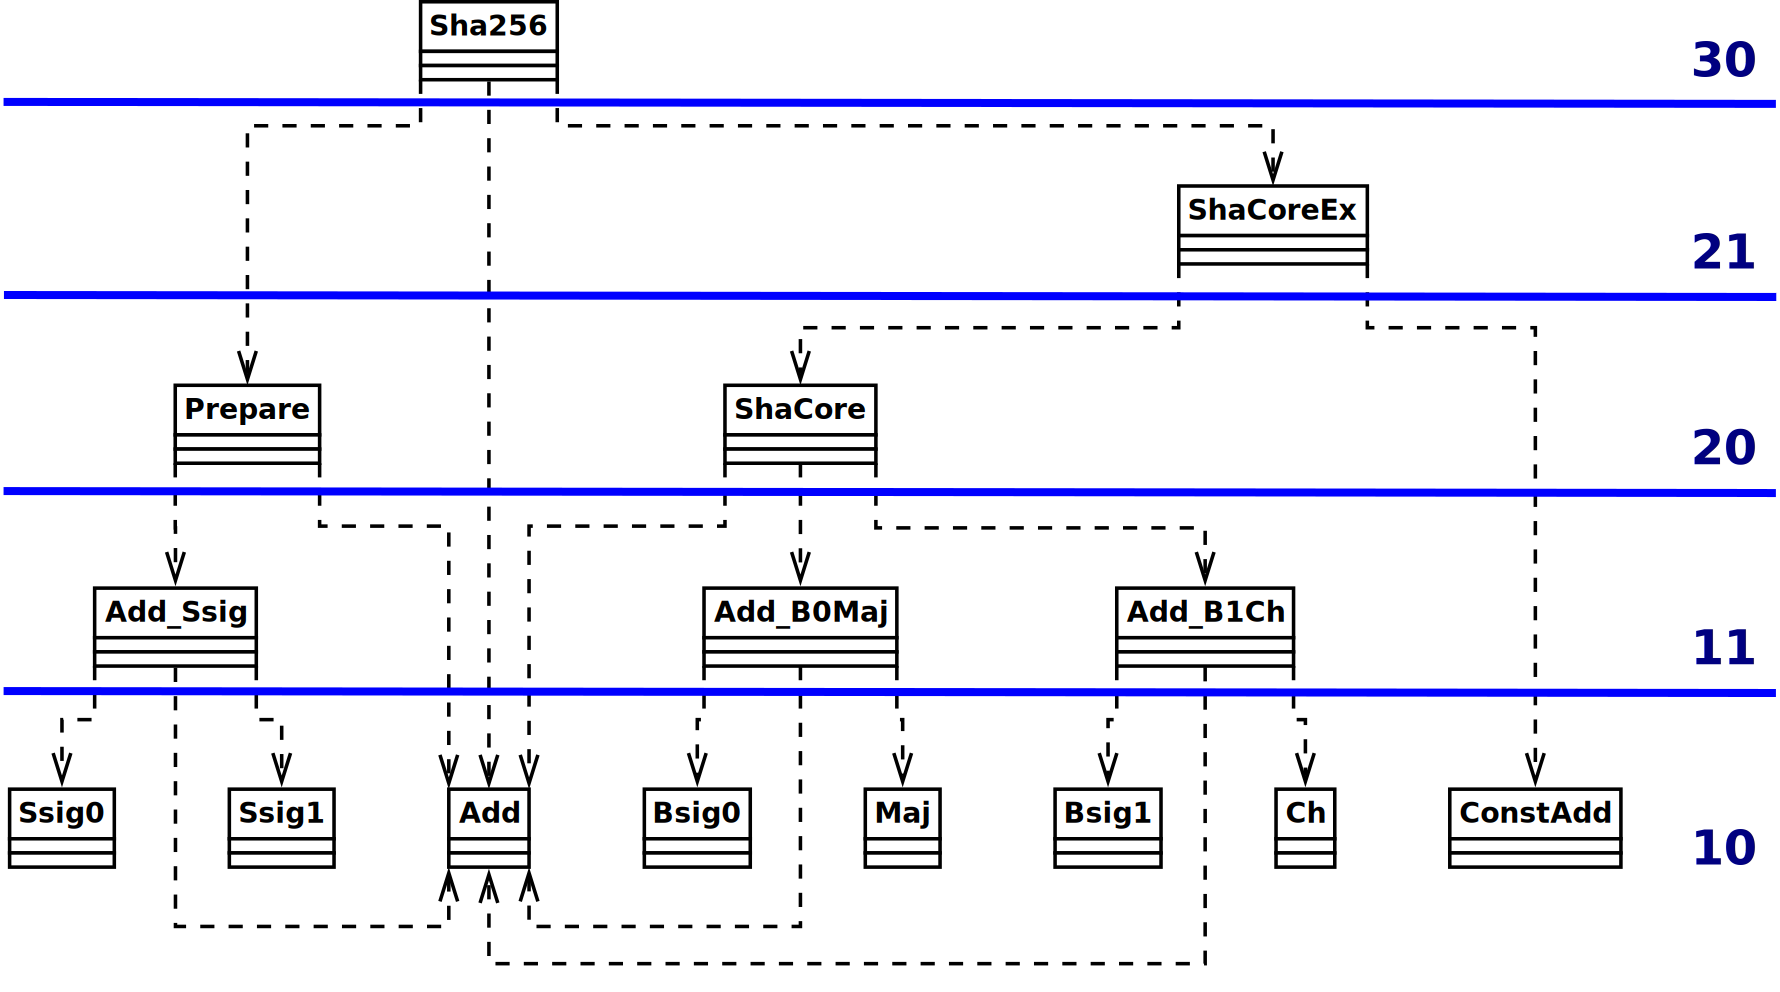
\includegraphics[scale=0.265]{images/module_level}
  \caption{Modullevel von \glos{sha256}}
  \label{fig:sha256_module_level}
\end{figure}

Die Level werden nicht fortlaufend nummeriert, um bei Bedarf weitere Module/Level einfügen zu können, ohne die Level der vorhandenen Module anpassen zu müssen.

Anhand der Level können die Module sortiert werden, so dass die Prüfung, ob eine Klausel zum Modul gehört, bei den Modulen mit dem niedrigsten Level beginnen kann.
Eine Klausel gehört dann zu einem Modul, wenn alle Literale der Klausel im Modul verwendet werden. Dabei kann es sich um Eingänge, zusätzliche Literale oder Ausgänge
handeln. Ein Sonderfall ist eine Klausel die ausschließlich aus Eingangsliteralen oder ausschließlich aus Ausgangsliteralen besteht. Die Ausgangsliterale eines Moduls
sind im allgemeinen die Eingangsliterale eines anderen Moduls wodurch die Zuordnung bei gleichem Level unklar ist. Klauseln dieser Art wurden bei der Analyse jedoch
nicht gefunden. 

Für die Zuordnung der Klauseln wird zunächst ein Collector mit dem Namen "`ModulDB"' implementiert. Die ModulDB überschreibt nur die Methode newModul des Collectors,
um die Registrierung der Module zu erfassen. Generierte Klauseln, die an die Methode create übergeben werden, werden dadurch ignoriert. Erfasst werden neben dem
Modulnamen und dem Level die verwendeten Literale in der Reihenfolge: Eingänge, zusätzliche Literale und Ausgänge. ModulDB stellt außerdem eine Funktion bereit,
der eine beliebige Klausel zur Zuordnung übergeben werden kann. Wird ein passendes Modul gefunden, wird ein Zeiger auf die Modulinformationen zurückgeliefert.

Das Programm "`modulchecker"' nutzt schließlich die ModulDB für die Zuordnung. Zunächst wird ein Objekt der Kompressionsfunktion erzeugt, in das die ModulDB als
Besucher übergeben wird. Danach werden die im vorigen Abschnitt erstellten DIMACS-Dateien eingelesen und jede Klausel einem Modul zugeordnet. Die Zuordnung wird
in diesem Fall immer gelingen, da spätestens die Kompressionsfunktion alle Literale umfasst.

Da die Module in ihrer Normalform implementiert werden (siehe Kapitel \ref{chp:knf}) kann eine zugeordnete Klausel noch nicht direkt genutzt werden.
Die verwendeten Literale in der Kompressionsfunktion sind andere als die des Moduls in der Normalform. Wird eine Klausel zugeordnet, erfolgt deshalb
direkt im Anschluss die Normalisierung der Klausel. Diese wird auf Basis der im Modul verwendeten Literale durchgeführt. Da diese in der richtigen
Reihenfolge vorliegen, können in der Klausel vorkommende Literale darin erkannt und anhand des Index in das Literal der Normalform überführt werden.

Nach der Normalisierung werden die Klauseln für jedes Modul in einem eigenen "`set"' gesammelt. Wie in Abschnitt \ref{sec:ana:rem_double} erfolgt
dadurch automatisch aussortierung doppel \TODO{hmm}.

mehrfach erkannt - set - wird aussortiert.


Programm "`clausechecker"' : testen der klauseln : vielleicht ungültig.


\begin{figure}[!h]
  \centering
  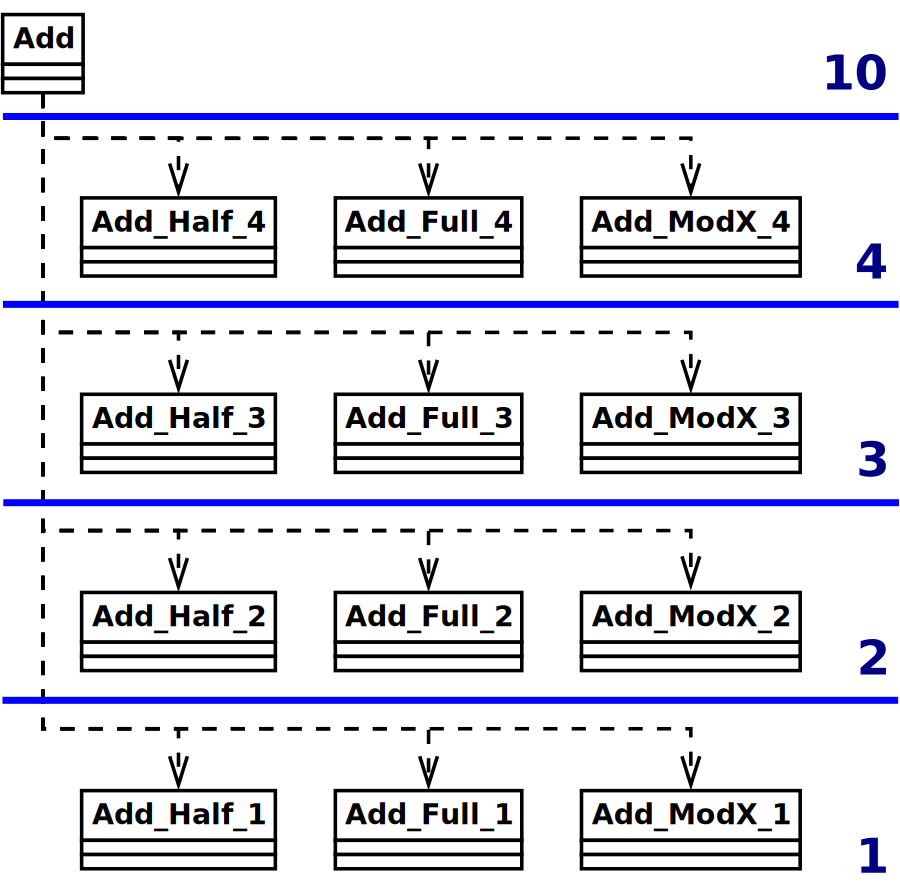
\includegraphics[scale=0.265]{images/module_add}
  \caption{Ergänzte Module von \glos{sha256}}
  \label{fig:sha256_module_add}
\end{figure}


\TODO{erledigen}


\section{Distanzermittlung von Klauseln in der Kompressionsfunktion}
\label{sec:ana:distance}

Die Analyse der neuen Klauseln aus der Kompressionsfunktion erfolgt auf Basis einer Distanzmetrik. Je höher die Distanz einer Klausel, desto höher
ist ihr angenommener Wert. Eine hohe Distanz bedeutet, dass die Klausel Literale aus Modulen in Zusammenhang bringt, die bisher in keiner direkten
Beziehung stehen.

Für die Distanzberechnung wird ein ungerichteter Graph aus den Modulen mit Level zehn erstellt. Ein Modul definiert sich dabei aus zusätzliche Literalen
und den Ausgangsliteralen. Im Gegensatz zum letzten Abschnitt fallen die Eingangsliterale weg, um eine eindeutige Zuordnung eines Literals zu einem
Modul durchführen zu können. Realisiert wird der Graph durch einen Collector mit dem Namen "`ModulGraph"'. Genau wie die ModulDB aus dem letzten Abschnitt
überschreibt der ModulGraph nur die Methode newModul des Collectors, um die Registrierung der Module zu erfassen. Um die Zuordnung der Literale zu einem
Modul schnellstmöglich durchführen zu können, wird eine Lookup-Tabelle erstellt, in der zu jedem Literal das zugehörige Modul hinterlegt ist. Registriert
sich ein Modul im ModulGraph, erfolgt zunächst die Aufnahme in die Lookup-Tabelle. Direkt im Anschluss wird das Modul mit den Modulen verknüpft, die die
Eingangswerte liefern, und so der ungerichtete Graph erstellt.

Der ModulGraph stellt eine Funktion "`printGraph"' bereit, mit der der ungerichtete Graph visualisiert werden kann. Die Ausgabe erfolgt in der Sprache DOT \cite{lang:dot}
mit der Graphen einfach beschrieben werden können. Mit Hilfe eines Renderes kann die Beschreibung des Graphen in ein Grafikformat überführt werden.
Optional kann als Parameter eine Klausel übergeben werden um Module, deren Literale in der Klausel vorkommen, farblich hervorzuheben. Abbildung \ref{fig:sha256_graph}
zeigt einen Ausschnitt aus dem vollständigen Graphen der Kompressionsfunktion. Abgebildet ist die dritte Anwendung der Rundenfunktion. Neben den
Modulnamen werden die verwendeten Literale ausgegeben. Da der Addierer zusätzliche Literale benötigt (Carrybits), sind bei diesem zwei Bereiche aufgeführt.
Die anderen Module kommen ohne zusätzliche Literale aus und enthalten somit nur die Ausgangsliterale. Anzumerken sind die fünf ausgehenden Kanten der beiden
finalen Addierer der Rundenfunktion. Die Ergebnisse werden jeweils in den vier folgenden Runden in fünf weiteren Modulen verwendet.
\begin{figure}[!h]
  \centering
  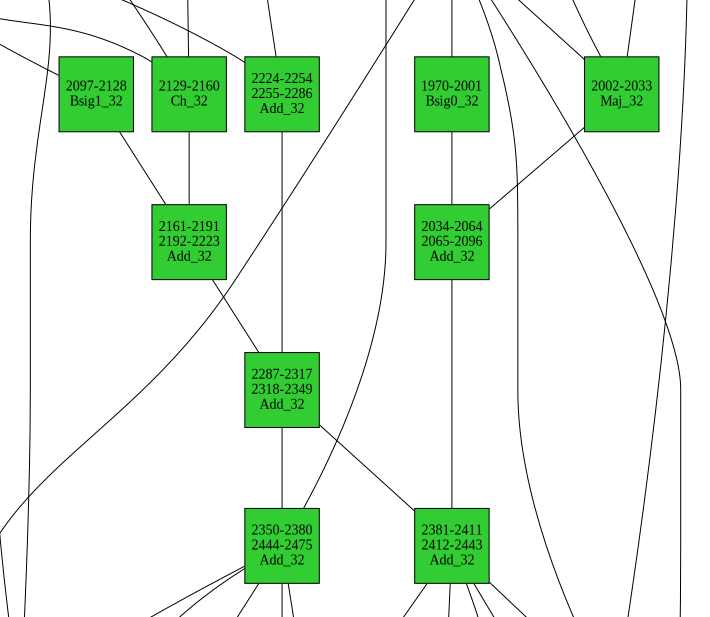
\includegraphics[scale=0.43]{images/sha256graph}
  \caption{Ausschnitt des ungerichteten Graphen von \glos{sha256}}
  \label{fig:sha256_graph}
\end{figure}

Nach der Erstellung des Graphs werden die Distanzen der Module untereinander berechnet. Für jedes Modul wird dafür der Dijkstra-Algorithmus \cite{dijkstra} angewandt,
um die Distanzen zu allen anderen Modulen zu berechnen. Jede Kante bekommt dabei das Gewicht eins. Genau wie für die Zuordnung der Literale zu den Modulen wird für
die Distanzermittlung eine Lookup-Tabelle verwendet. In jedem Knoten werden so die Distanzen zu allen anderen Modulen abgelegt. Für die vollständige Kompressionsfunktion
von \glos{sha256} stellt sich heraus, dass die größte Distanz zwischen zwei Modulen sechzehn beträgt; Es liegen somit maximal fünfzehn Module zwischen zwei anderen
Modulen. Berechnet werden durch den Dijkstra-Algorithmus auch die Wege für die die Distanz gilt. Die Wege haben jedoch für diese Arbeit keine Relevanz und werden
verworfen. Durch die Lookup-Tabellen kann die Berechnung der Distanzen einmalig bei Programmstart erledigt werden und große Klauselmengen können effizient bewertet werden.

Nachdem die Distanzen der einzelnen Module bekannt sind, kann damit die Distanz einer Klausel berechnet werden. Da eine Klausel mehr als zwei Module betreffen kann, werden
die Distanzen aller betroffenen Module überprüft und die größte Distanz ausgewählt. Ermittelt wird außerdem die Anzahl der betroffenen Module. Ein Klausel mit sechs Literalen
kann zum Beispiel zwei Module betreffen, wenn je drei Literale aus einem Modul stammen. Die Distanz einer Klausel ergibt sich aus der Formel in Abbildung \ref{eq:clausedistance}.
\begin{figure}[!h]
  \begin{align*}
  Klauseldistanz = gr\ddot{o}{\beta}te~Moduldistanz - Modulanzahl + 1
  \end{align*}
  \caption{Formel zur Berechnung der Distanz einer Klausel}
  \label{eq:clausedistance}
\end{figure}

Die Formel soll anhand eines Beispiels erläutert werden bei dem eine Klausel mit vier Literalen herangezogen wird. Die Zuordnung der Literale
zu den Modulen ergibt drei unterschiedliche Module. Bei dem Vergleich der Distanzen zwischen den Modulen wird eine maximale Distanz von drei ermittelt.
Mit der Formel aus Abbildung \ref{eq:clausedistance} ergibt sich eine Klauseldistanz von eins.

Abbildung \ref{fig:distance} zeigt zwei mögliche Fälle, die dem Beispiel entsprechen. In den gezeigten Graphen sind die Module, denen mindestens ein Literal
zugeordnet wurde rot eingefärbt. Weitere Module denen kein Literal der Klausel zugeordnet werden konnte, sind in grün dargestellt.
\begin{figure}[!h]
  \centering
  \begin{minipage}[b]{6cm}
    \centering
    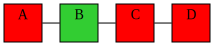
\includegraphics[scale=0.6]{images/distance1}\\
    Schlechtester Fall
  \end{minipage}
  \begin{minipage}[b]{6cm}
    \centering
    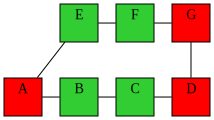
\includegraphics[scale=0.6]{images/distance2}\\
    Weiterer Fall
  \end{minipage}
  \caption{Beispiel für die Distanz einer Klausel}
  \label{fig:distance}
\end{figure}

Im schlechtesten Fall ergibt sich die maximale Distanz zwischen den Modulen A und D, wobei das dritte Modul C auf dem Pfad zwischen den Modulen A und D liegt.
Genau ein Modul B wird dabei übersprungen, was genau dem Wert der Klauseldistanz entspricht. Die Klauseldistanz sagt damit aus, wie viele Module im schlechtesten
Fall übersprungen werden.

Ein weiterer Fall zeigt, dass die Klauseldistanz auch höher sein kann, wenn weitere Pfade von Modul A nach Modul D führen. Ein weiterer Pfad ist jedoch mindestens
genau so lang wie der erste Pfad. Angenommen der zusätzliche Pfad hat die Länge vier und das dritte betroffenen Modul (in diesem Fall G) liegt auf diesem längeren
Pfad, werden zwei Module übersprungen.

Um die Distanz für die neuen Klauseln aus der Kompressionsfunktion zu ermitteln, wird das Programm "`distancechecker"' erstellt. Dieses Programm liest alle Klauseln
ein und verteilt diese je nach Klauseldistanz auf eine eigene DIMACS-Datei. Vernachlässigt wird bei diesem Vorgehen die Länge der Klausel. Die Anzahl der Literale
wird nur indirekt durch die Anzahl der betroffenen Module berücksichtigt. Dies wird aber vernachlässigt, da Klauseln mit großer Länge und Distanz durchaus interessant
sein könnten, auch wenn es eher unwahrscheinlich ist, dass sie den Lösungsprozess in CryptoMiniSat beschleunigen.

Bei der Analyse zeigt sich, dass die Distanz der Klauseln breit gestreut ist. Die Distanz reicht von $5$ bis unter $-250$. Wird zum Vergleich eine Klausel betrachtet,
die einem einzelnen Modul mit Level zehn zugeordnet ist, ergibt sich dafür eine Klauseldistanz von $0$ ($= 0 - 1 + 1$). Darauf basierend werden im weiteren Verlauf
nur Klauseln berücksichtigt, deren Distanz größer als null ist, in der Erwartung, dass sie zusätzliches Wissen darstellen und den Lösungsprozess beschleunigen.
\section{Verallgemeinerung von Klauseln}
\label{sec:ana:generalize}

Bisher erhaltene Klauseln werden in diesem Abschnitt darauf untersucht, ob eine Verallgemeinerung möglich ist. Verallgemeinerung bedeutet dabei, den Sinn der Klausel
zu erkennen und auf weitere Stellen anzuwenden. Auf Modulebene erfolgt dieser Prozess bereits automatisch, da diese Klauseln überall dort angewendet werden, wo das
Modul zum Einsatz kommt. Eine weitere Möglichkeit ist es, weitere Stellen innerhalb des Moduls zu identifizieren, an denen die Klausel ebenfalls gültig ist. Besonders
gut funktioniert diese Verallgemeinerung bei dem Addierer. Durch die Breite von 32 Bit können viele Klauseln bitweise nach vorne oder hinten verschoben werden und sind
an diesen Stellen ebenfalls gültig. Aufgrund der Vielzahl der erhaltenen Klauseln ist jedoch eine weitere Unterteilung notwendig. Zunächst werden die in Abschnitt
\ref{sec:knf:addierer} erläuterten Komponenten des Addierers (Halb-, Voll- und Mod-2 Addierer) in eigene Module mit dem Level eins ausgelagert. Dadurch können viele
Klauseln direkt den Halb-, Voll und Mod-2 Addiereren zugeordnet werden. Ein Großteil der erworbenen Klauseln verbleibt aber nach wie vor im Modul des 32-Bit Addierers.
Bei der Analyse der verbleibenden Klauseln zeigt sich, dass sich diese Klauseln in Halb-, Voll und Mod-2 Addiereren höherer Ebene organisieren lassen. Als Addierer
höherer Ebene wird ein Addierer bezeichnet, der bei Bedarf ein eingehendes oder ausgehendes Carrybit berücksichtigt, intern jedoch keine Carrybits verwendet. Diese
Addierer entsprechen dem Carry-Lookahead Addierer (siehe Abschnitt \ref{sec:grundlagen_add}) in unterschiedlichen Bitbreiten. Ergänzt werden Module für Addierer bis
vier Bit Breite. Abbildung \ref{fig:sha256_module_add} zeigt die Erweiterung der Modulhierarchie.
\begin{figure}[!h]
  \centering
  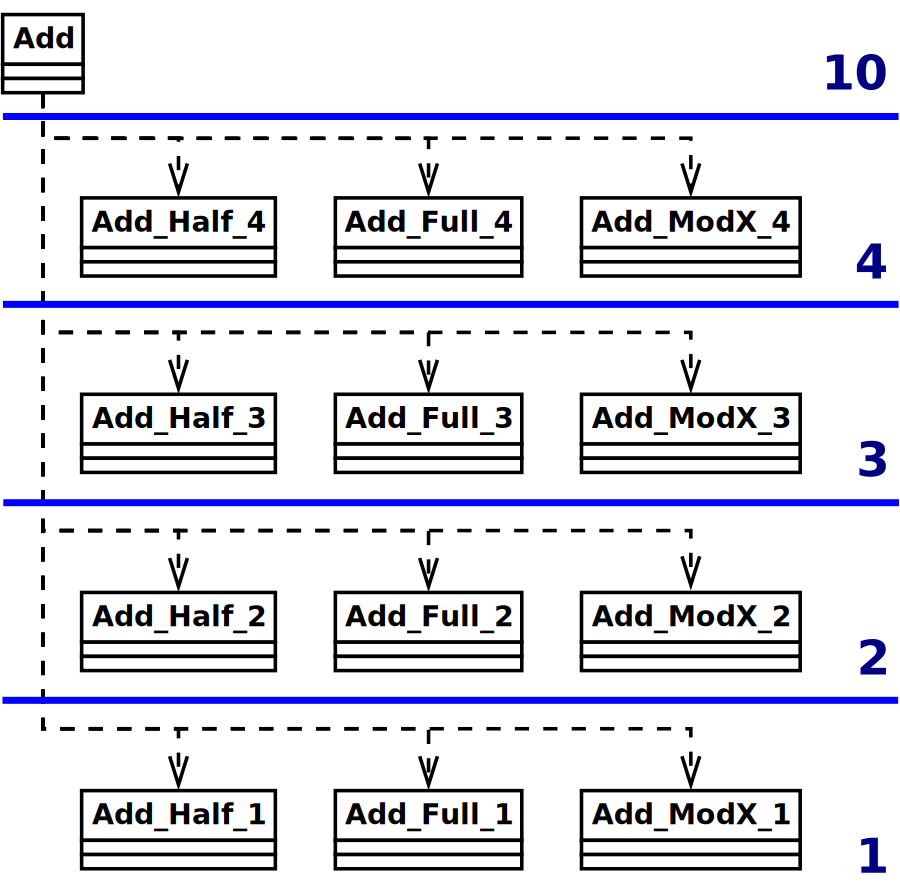
\includegraphics[scale=0.265]{images/module_add}
  \caption{Ergänzte Module von \glos{sha256}}
  \label{fig:sha256_module_add}
\end{figure}

Module für Addierer mit mehr als vier Bit Breite werden nicht ergänzt, da der SAT-Solver keine Klauseln ermittelt hat, die diesen Modulen zugeordnet werden könnten.  
Notwendig für die Funktion des Addierers sind nur die Module mit dem Level eins. Die Module mit dem Level zwei bis vier dienen als zusätzliche Information
auf den selben Literalen. Durch dieses Vorgehen erfolgt die Verallgemeinerung von Klauseln innerhalb des Addierers ebenfalls automatisch.

Bei den anderen Modulen zeigt sich kein Muster dieser Art und die Anzahl der erworbenen Klauseln ist vergleichsweise gering. Deshalb werden die erworbene Klauseln
darin direkt untergebracht und durch Verwendung einer Schleife verallgemeinert in sofern dies möglich ist. Eine Ausnahme bildet das Modul der vollständigen
Kompressionsfunktion. Neben der Verallgemeinerung auf Bitbreite bietet sich in diesem Modul die Möglichkeit, die Klauseln auch auf weitere Runden anzuwenden.
Klauseln die sich nur auf eine Runde beziehen wurden schon dem Modul für die Rundenfunktion zugeordnet, so dass nur noch Klauseln betrachtet werden die sich über
zwei oder mehr Runden erstrecken. Jedes Literal der jeweiligen Klausel wird um eine Runde nach vorne oder hinten verschoben.

Beachtet werden muss, dass jede der 64 Runden eine andere Rundenkonstante verwendet und die Erweiterung der Eingabe bei den ersten 16 Runden keine
Anwendung findet. Während bei den anderen Modulen im Allgemeinen eine Verallgemeinerung entweder funktioniert oder nicht, muss dadurch jede durch die
Verallgemeinerung generierte Klausel einzeln überprüft werden. Wie auch bei der Überprüfung der modulspezifischen Klauseln in Abschnitt \ref{sec:ana:module}
wird das Programm "`clausechecker"' für die Überprüfung genutzt. Nur wenige der ermittelten Klauseln lassen sich ohne Einschränkungen auf weitere Bits oder
Runden übertragen. Der clausechecker generiert deshalb ein zweidimensionales Array, in dem die gültigen Klauseln markiert werden. Dieses Array wird im
Modul der Kompressionsfunktion genutzt, um die gültigen Klauseln zu generieren. Es zeigt sich, dass die Werte des Arrays in einigen Fällen die Rundenkonstante
widerspiegeln. Im diesem Fall wird auf das Array verzichtet und die Bits der Rundenkonstante verwendet.
\section{Erhaltene Klauseln}
\label{sec:ana:acquired}

generell anzahl gelernter klauseln angeben: auch werte über klausellängen

subklauseln sind enthalten: werte angeben

\TODO{erledigen}